\maketitle

\begin{abstract}
Simple Linux Utility for Resource Management (SLURM) is an open source,
fault-tolerant, and highly scalable cluster management and job 
scheduling system for Linux clusters of 
thousands of nodes.  Components include machine status, partition
management, job management, and scheduling modules.  The design also 
includes a scalable, general-purpose communication infrastructure.
Development will take place in four phases:  Phase I results in a solid
infrastructure;  Phase II produces a functional but limited interactive 
job initiation capability without use of the interconnect/switch; 
Phase III provides switch support and documentation; Phase IV provides 
job statusing, fault-tolerance, and job queuing and control through  
Livermore's Distributed Production Control System (DPCS), a meta-batch and
resource management system.
\end{abstract}

\vspace{0.25in}

%\begin{center}
%
\epsfig{file=slurm.eps,width=4in}
%\end{center}

\newpage



\section{Overview}

SLURM\footnote{A tip of the hat to Matt Groening and creators of {\em Futurama},
where Slurm is the highly addictive soda-like beverage made from worm
excrement.} (Simple Linux Utility for Resource Management) 
is a resource management 
system suitable for use on Linux clusters, large and small.  After 
surveying\cite{Jette2002} resource managers available for Linux and finding 
none that were simple, highly scalable, and portable to different cluster 
architectures and interconnects, the authors set out to design a new system.

The result is a resource management system with the following general
characteristics:

\begin{itemize}
\item {\em Simplicity}: SLURM is simple enough to allow motivated end users
to understand its source code and add functionality.  The authors will 
avoid the temptation to add features unless they are of general appeal.

\item {\em Open Source}: SLURM is available to everyone and will remain free;
its source code is distributed under the GNU General Public License.

\item {\em Portability}: SLURM is written in the C language, with a GNU 
autoconf configuration engine.  While initially written for Linux, 
other UNIX-like operating systems should be easy porting targets.

\item {\em Interconnect independence}: Initially, SLURM supports TCP/IP based
communication and the Quadrics Elan3 interconnect.  Adding support for other
interconnects is straightforward.  Users select the supported interconnects
at compile time via GNU autoconf.

\item {\em Scalability}: SLURM is designed for scalability to clusters of
thousands of nodes.\footnote{It is anticipated that a Linux cluster of
size $>1000$ nodes will be available for testing before the initial public 
release.}

\item {\em Fault tolerence}: SLURM can handle a variety of failure modes
without terminating workloads, including crashes of the node running the SLURM
controller.

\item {\em Secure}: SLURM employs crypto technology to authenticate 
users to services and services to services.  
A Kerberos v5 infrastructure can be utilized if available.
SLURM does not assume that its networks are physically secure.

\item {\em System administrator friendly}: SLURM is configured with a few
simple configuration files and minimizes distributed state.  Its interfaces
are scriptable and its behavior is highly deterministic.

\end{itemize}

\subsection{What is SLURM?}

As a cluster resource manager, SLURM has three key functions.  First,
it allocates exclusive access to resources (compute nodes) to users for 
some duration of time so they can perform work.  Second, it provides 
a framework for starting, executing, and monitoring work (normally a 
parallel job) on the set of allocated nodes.  Finally, it arbitrates 
conflicting requests for resources by managing batch queues.

Users interact with SLURM through three command line utilities: 
{\tt srun} for submitting a job for execution and optionally controlling it
interactively; 
{\tt scancel} for early termination of a job; 
and {\tt squeue} for monitoring queues.

System administrators perform privileged operations through an additional
command line utility: {\tt slurmadmin}.

External schedulers and meta-batch systems can submit jobs to SLURM and
order its queues through an application programming interface (API).

Compute nodes simply run a {\tt slurmd} daemon (similar to a remote shell 
daemon) to export control to SLURM.  The central controller daemon,
{\tt slurmctld}, maintains the global state and directs operations.

\subsection{What SLURM is Not}

SLURM is not a sophisticated batch system.  Its default scheduler
implements FIFO with backfill and does not include the bells and 
whistles needed to implement complex site policy.
SLURM does however provide a sufficiently sophisticated API for an external 
scheduler or meta-batch system to order its queues based on site policy.

SLURM clusters are space shared, and parallel jobs are always 
assigned whole nodes.  SLURM does not support gang scheduling (time-slicing 
of parallel jobs). However, the explicit preemption and later resumption 
of a job under the direction of an external meta-batch system may be supported 
in the future. At present, an external scheduler may terminate jobs and 
requeue them in a different order via the API. 

SLURM is not a meta-batch system like Globus or DPCS (Distributed Production 
Control System).  SLURM supports resource management across a single cluster.

SLURM is not a comprehensive cluster administration or monitoring package.  
While SLURM knows the state of its compute nodes, it makes no attempt to put
this information to use in other ways, such as with a general purpose event
logging mechanism or a back-end database for recording historical state.
It is expected that SLURM will be deployed in a cluster along side other 
tools that perform these functions. 

\subsection{Architecture}

\begin{figure}[htb]
\centerline{\epsfig{file=arch.eps}}
\caption{SLURM Architecture}
\label{arch}
\end{figure}

\begin{figure}[htb]
\centerline{\epsfig{file=LCM.arch.eps,scale=0.5}}
\caption{SLURM Architecture - Subsystems}
\label{archdetail}
\end{figure}


As depicted in Figure~\ref{arch}, SLURM consists of 
a {\tt slurmd} daemon running on each compute node, 
a central {\tt slurmctld} daemon running on a management node (with optional 
failover twin), 
and a four command line utilities: {\tt srun}, {\tt scancel}, {\tt squeue}, 
and {\tt slurmadmin}, which can run anywhere in the cluster.
A scalable communications library ties these components together.

Figure~\ref{archdetail} exposes the subsystems that are implemented within
the {\tt slurmd} and {\tt slurmctld} daemons.  These subsystems are explained
in more detail below.

\subsubsection{Slurmd}

The {\tt slurmd} running
on each compute node can be compared to a remote shell daemon:  it waits 
for work, executes the work, returns status, then waits for more work.  
It also asynchronously exchanges node and job status with the controller.  
It never communicates with other compute nodes and the only job information 
it has at any given time pertains to the currently executing job.

{\tt slurmd} reads its configuration from a file: {\tt /etc/slurmd.conf}
and has three major components:

\begin{itemize}
\item {\em Machine and Job Status Service}:  Respond to controller 
requests for machine and job state information, and send asynchronous 
reports of some state changes (e.g. {\tt slurmd} startup, process 
termination) to the controller.
Job status includes CPU, real-memory and virtual memory consumption 
information for all processes including user processes, system daemons, 
and the kernel. 

\item{\em Process Manager}:  Start, monitor,signal, and clean up after
a set of processes belonging to a parallel job, as dictated by the
controller.  Starting a process may include executing a prolog script, 
setting process limits, setting real and effective
user id, setting environment, setting current working directory, allocating 
interconnect resources, setting core paths, and managing process groups.  
Terminating a process may include terminating all members of a process 
group, and executing an epilog script.

\item{\em Stream Copy Service}:  Allow stderr/stdout/stdin and core files
to be copied in and out of the spool directory for a job.  In the case
of batch jobs, this will happen during startup and cleanup only and will
occur between the controller and {\tt slurmd}'s.
In the case of interactive jobs, stdout/stderr may additionally be ``carbon 
copied'' to the {\tt srun} command during job execution.

\end{itemize}

\subsubsection{Controller}

Most SLURM state exists in the controller, {\tt slurmctld}. 
When {\tt slurmctld} starts, it reads its configuration from a file:
{\tt /etc/slurmctld.conf}.  It also can read additional state from a 
checkpoint file left over from a previous {\tt slurmctld}.
{\tt slurmctld} runs in either master or standby mode, depending
on the state of its failover twin, if any.  

{\tt slurmctld} performs several tasks simultaneously:

\begin{itemize}
\item {\em Partition Manager}: Monitors the state of each 
node in the cluster.  It polls {\tt slurmd}'s for status periodically and 
receives state change notifications from {\tt slurmd}'s asynchronously.
The partition manager groups nodes into non-overlapping sets 
called {\em partitions}. Each partition can have associated with 
it various job limits and access controls.
The partition manager also allocates nodes to jobs based upon 
node and partition states and configurations. Requests to initiate 
jobs come from the Job Manager.
{\tt slurmadmin} may be used to administratively alter node and 
partition configurations.

\item {\em Job Manager}: Accepts user job requests and (if applicable) 
places pending jobs in a priority ordered queue. By default the job 
priority will be a simple age based algorithm providing FCFS ordering. 
An interface is provided for an external scheduler to establish 
a job's initial priority and API's are available to alter this priority 
through time for customers wishing a more sophisticated algorithm.
The job manager is awakened whenever there is a change in state that 
might permit a job to begin running, such as job completion, job submission, 
partition {\em up} transition, or node {\em up} transition.
The job manager then makes a pass through the job queue and
starts jobs until a resource allocation fails. 
When a resource allocation failure occurs, the Job Manager establishes 
a time when the job might be expected to begin execution. 
Lower priority jobs in the queue will be allocated resources on that 
partition only if they will complete prior to the expected initiation 
time of the higher priority job (backfill scheduling).
After completing the scheduling cycle, the job manager's scheduling 
thread sleeps.
Once a job has been allocated resources, the job manager transfers 
necessary state information to those nodes and commences its execution. 
Once executing, the job manager will monitor and record the job's resource 
consumption (CPU cycles, real memory, and virtual memory) in near realtime.
When the job manager detects that all nodes associated with a 
job have completed their work, it initiates cleanup and performs a 
scheduling cycle as described above.

\item {\em Switch Manager}:  Monitor the state of interconnect links 
and inform the machine status manager of any compute nodes whose links
have failed.  The switch manager can be configured
to use Simple Network Monitoring Protocol (SNMP) to obtain link
information from SNMP-capable network hardware.
The switch manager configuration is optional;  without one, 
SLURM simply ignores link errors.

\end{itemize}

\subsubsection{Command Line Utilities}

The command line utilities primarily interact with the controller.
The utilities find the host:port of the controller by reading a configuration 
file: {\tt /etc/slurm.conf}.
They authenticate to the controller using a method selected at compile
time, initially either Kerberos v5 or ...?

\marginpar{Chris help me out here on the authentication --JG}

\begin{itemize}
\item {\tt srun}: Submit a job for execution.  {\tt srun} may run in either
interactive or batch mode.  {\tt srun}'s standard input (if it is a file) is 
copied to the controller, which copies it to {\tt slurmd}'s\footnote{{\tt srun}
command line options select the stdin handling method such as broadcast to 
all tasks, or send only to task 0.}
After job submission, batch {\tt srun} terminates, while interactive 
{\tt srun} establishes connections with {\tt slurmd}'s to get standard output 
and error of the tasks in real time, and responds to signals from the 
user.\footnote{From the controller's point of view there is no difference 
between batch and interactive jobs;  an interactive {\tt srun} may detach from 
its job, leaving it to continue running as though submitted in batch mode.
It is also possible for {\tt srun} to attach to a job interactively that
was submitted in batch mode, subject to authentication.}

\item {\tt squeue}: Display the queue of running and waiting jobs.

\item {\tt scancel}: Cancel a running or a waiting job, subject to
authentication.

\item {\tt slurmadmin}: Perform privileged administrative commands
such as draining a partition in preparation for maintenance, or terminating
jobs.  Must be run as the root user.

\end{itemize}

\subsubsection{Communications Layer}

{\em Does the communications layer need to handle stdout/stderr streams?
If these only apply to an interactive run, can we live with TCP?
TCP may also be appropriate for the copying of stdout/stderr/stdin/core
at the beginning and end of a job.  If that requirement is lifted,
the comm layer design over UDP is simpler.}

\subsection{Example:  Executing a Batch Job}

A user wishes to run a job in batch mode, in which {\tt srun} will return 
immediately and the job will execute ``in the background'' when resources
are available.

The job is a two-node run of {\em mping}, a simple MPI application.
The user submits the job:
\begin{verbatim}
srun --batch --nodes 2 --nprocs 2 1 mping 1 1048576
\end{verbatim}

The {\tt srun} command authenticates the user to the controller and submits
the job request.  As stdin is not a file, it is not copied to the controller.
The request includes the {\tt srun} environment, current working directory, 
and command line option information.

The controller consults the partition manager to test whether the job will
will ever be able to run.  If the user has requested a non-existent partition,
more nodes than are configured in the partition, a non-existent constraint, 
etc., the partition manager returns an error and the request is discarded.
The failure is reported to {\tt srun} which tells the user and exits:
\begin{verbatim}
srun: request will never run
\end{verbatim}

On successful submission, the controller assigns the job a unique 
{\em batch id}, adds it to the job queue and returns the 
batch id to {\tt srun}, which reports this to user and exits, returning
success to the user's shell:

\begin{verbatim}
srun: tinymem-42
\end{verbatim}

The controller awakens the job manager which tries to run
jobs starting at the head of the job queue.  It finds {\em tinymem-42}
and makes a successful request to the partition manager to allocate 
two nodes from the {\em tinymem} partition: {\em dev6} and {\em dev7}.

The job manager sends a copy of the environment, current working directory,
command path, command arguments, interconnect info, etc.
to the {\tt slurmd}'s running on {\em dev6} and {\em dev7}.  
The {\tt slurmd}'s set up the environment and execute the command as 
the submitting user.  Stdout and stderr are redirected to files on the 
compute nodes:

\begin{verbatim}
/var/spool/slurm/tinymem-42/stdout.[mpirank]
/var/spool/slurm/tinymem-42/stderr.[mpirank]
\end{verbatim}

The job manager continues trying to initiate jobs until it cannot, then sleeps.
Meanwhile, on {\em dev6}, {\tt /var/spool/slurm/tinymem-42/stdout.0}
accumulates the application's output:

\begin{verbatim}
  1 pinged   0:        1 bytes      5.38 uSec     0.19 MB/s                     
  1 pinged   0:        2 bytes      5.32 uSec     0.38 MB/s                     
  1 pinged   0:        4 bytes      5.27 uSec     0.76 MB/s                     
  1 pinged   0:        8 bytes      5.39 uSec     1.48 MB/s                     
  ...
  1 pinged   0:  1048576 bytes   4682.97 uSec   223.91 MB/s              
\end{verbatim}

When all tasks complete, the {\tt slurmd}'s on the two compute nodes notify
the job manager, which changes the job status to {\em stage\_out} and begins cleanup.
It retrieves the stdout/stderr spool files from the stream copy service
of each {\tt slurmd} and merges them into a single report, 
which it stores in the user's {\tt srun} directory.
It directs the slurmd daemon on each of the nodes formerly assigned to the 
job to execute the epilog commands (if any).
Finally, the job manager releases resources and changes the job's state to 
{\em complete}. The records of a job's existence will eventually be purged.


\subsection{Example:  Executing an Interactive Job}

A user wishes to run the same job in interactive mode, in which {\tt srun}
will block while the job executes and stdout/stderr of the job will be 
copied onto stdout/stderr of {\tt srun}.

The user submits the job, this time requesting an interactive run:
\begin{verbatim}
srun --nodes 2 --nprocs 2 1 mping 1 1048576
\end{verbatim}

The {\tt srun} command authenticates the user to the controller and 
executes the same steps described in the batch example, except {\tt srun} 
does not terminate on successful submission.  Instead, it receives a list of
hostnames and a {\em nonce} used to authenticate to the {\tt slurmd}'s.
After the job startup, {\tt srun} has no further interaction with the 
controller.

{\tt srun} then opens connections to the {\tt slurmd}'s and copies 
stdout/stderr of each task to stdout/stderr of {\tt srun}.  These streams
are also spooled on the node and will be collected, merged, and stored
in the user's {\tt srun} directory on completion.

The user sees the output of task 0 on stdout of {\tt srun}:

\begin{verbatim}
  1 pinged   0:        1 bytes      5.38 uSec     0.19 MB/s                     
  1 pinged   0:        2 bytes      5.32 uSec     0.38 MB/s                     
  1 pinged   0:        4 bytes      5.27 uSec     0.76 MB/s                     
  1 pinged   0:        8 bytes      5.39 uSec     1.48 MB/s                     
  ...
  1 pinged   0:  1048576 bytes   4682.97 uSec   223.91 MB/s              
\end{verbatim}

When the job terminates, {\tt srun} receives an EOF on each stream and
closes them, gets the job exit status from {\tt slurmd}'s, and terminates.

If a signal is received by {\tt srun} while the job is executing (for example,
a SIGINT resulting from a Control-C), it is sent to each {\tt slurmd} which 
terminates the individual tasks and reports this to the job status manager,
which cleans up the job.

\marginpar{This is as far as I got in the ``big picture'' update --JG}

\section{Controller Design}

The controller will be modular and multi-threaded. 
Independent read and write locks will be provided for the various data 
structures for scalability. 
The controller  will include the following subsystems:

\begin{itemize}
\item {\em Partition management}: Monitor and record the state of each 
node in the cluster.
Group these nodes into disjoint sets called {\em partitions} with various 
job limits and access controls.
The partition manager also allocates nodes to jobs based upon 
node and partition states and configurations. 

\item {\em Job management}: Accept, initiate, monitor, delete and otherwise 
manage the state of all jobs in the system. This includes the prioritization 
of pending work.

\item {\em Switch management}: Perform any interconnect-related 
monitoring and control needed to run a parallel job.

\end{itemize}

Each of these subsystems is described in detail below.

\subsection{Partition Management}

The partition manager will monitor the sate of nodes and allocate 
these resources to jobs selected by the Job Manager. 
Node information that we intend to monitor includes:

\begin{itemize}
\item Count of processors on the node
\item Size of real memory on the node
\item Size of temporary disk storage
\item State of node (RUN, IDLE, DRAIN, etc.)
\end{itemize}

The SLURM administrator could at a minimum specify a list of system node 
names using a regular expression (e.g. "NodeName=linux[001-512] CPUs=4 
RealMemory=1024 TmpDisk=4096"). 
This would be considered the minimal node configuration values which are 
acceptable for the node to enter into service.

The partition manager will identify groups of nodes to be used for
execution of user jobs. Data to be associated with a partition will include:
\begin{itemize}
\item Name
\item Access controlled by key granted to key (so support external schedulers)
\item List of associated nodes
\item State of partition (UP or DOWN)
\item Maximum time limit for any job
\item Maximum nodes allocated to any single job
\item List of groups permitted to use the partition (defaults to ALL)
\end{itemize}

It will be possible to alter this data in real-time in order to effect the
scheduling of pending jobs (currently executing jobs would continue). Unlike some
other parallel job management systems, we believe this information can be
confined to the SLURM control machine for better scalability. It would be used
by the Job Manager (and possibly an external scheduler), which either exist only 
on the control machine or communicate only with the control machine. An API to 
manage this information would be developed first, followed by a simple command-line 
tool utilizing the API.

The partition manager will allocate nodes to pending jobs upon request by 
the job manager. 
The current SLURM design only supports the allocation of entire nodes to 
jobs. Our customers at LLNL have expressed the opinion that sharing of 
nodes can severely reduce their job's performance and even reliability. 
This is due to contention for shared resources such as local disk space, 
real memory, virtual memory and processor cycles. The proper support of 
shared resources, including the enforcement of limits on these resources, 
entails a substantial amount of additional effort. Given such a cost to 
benefit situation at LLNL, we have decided to not support shared nodes. 
However, we have designed SLURM so as to not preclude the addition of 
such a capability at a later time if so desired.
Future enhancements could include constraining jobs to a specific CPU count 
or memory size within a node, which could be used to space-share the node.

\subsection{Job Manager}

The core functions to be supported by the job manager include:
\begin{itemize}
\item Queue job request
\item Order job queue (under control of external scheduler)
\item Initiate job
\item Will job run query (test if "Initiate job" request would succeed)
\item Status job (including node list, memory and CPU use data)
\item Signal job for termination (following DPCS model of explicit application
registration)
\item Terminate job (remove all processes)
\item Preempt/resume job  (future)
\item Checkpoint/restart job (future)
\item Change node count of running job (could fail if insufficient resources are 
available, future)
\end{itemize}

Submitted jobs can specify desired partition, CPU count, node count, task 
count, task distribution pattern (round-robin or sequential within a node), 
and (optionally) an explicit list of nodes. The submitted job may have an 
associated key, and by virtue of this can be granted access to specific partitions. 

We propose that SLURM implement a very simple scheduling algorithm, 
namely First-in First-out (FIFO) with backfill. Backfill scheduling 
means that a lower priority job (i.e. newer) can be scheduled before 
another job only if doing so does not delay the expected initiation 
time of the higher priority job. Backfill scheduling tends to improve 
both system utilization and responsiveness by initiating smaller 
node count and shorter time limit jobs more rapidly. 

We are well aware this algorithm will not satisfy the needs of many 
customers and provide the means for establishing other scheduling 
algorithms. Before a newly arrived job is placed into the queue, it 
is assigned a priority that may be established by an administrator 
defined program. SLURM APIs permit an external entity to alter the 
priorities of jobs at any time to re-order the queue as desired. 
The Maui Scheduler\footnote{http://mauischeduler.sourceforge.net/} 
is one example of an external scheduler suitable for use with SLURM.

A more sophisticated scheduler that we plan to offer with SLURM is 
DPCS\footnote{http://www.llnl.gov/icc/lc/dpcs/dpcs\_overview.html}. 
DPCS has flexible scheduling algorithms that suit our needs well and
provide the scalability required for this application. Most of the resource
accounting and some of the job management functions presently within DPCS would
be moved into the proposed SLURM Job Management and Job Status components. 
DPCS will require some modification to operate within this new, richer
environment. The DPCS Central Manager would also require porting to Linux. 

The DPCS writes job accounting records to Unix files. Presently, these are
moved to a machine with the Sybase database. This data can be accessed via
command-line and web interfaces with Kerberos authentication and authorization.
We are not contemplating making this database software available through SLURM,
but might consider writing this data to an open source database if so desired.

System specific scripts can be executed prior to the initiation of a user job
and after the termination of a user job (e.g. prolog and epilog). These scripts
can be used to establish an appropriate environment for the user (e.g. permit
logins, disable logins, terminate "orphan" processes, etc.). 
An API for all functions would be developed initially, followed by a  
command-line tool utilizing the API. 

\subsection{Switch Manager}

The switch manager would be responsible for allocating switch channels and assigning 
them to user jobs. The switch channels would be de-allocated upon job termination. 
The slurmd (on each compute node) would provide user jobs with the authentication 
required for switch use as directed by the switch manager. Switch health monitoring tools will 
also be implemented in phase two. It may be desirable for the SLURM daemons to use the
switch directly for communications, particularly for the movement of a large 
executable and/or standard input file. This option will be investigated in phase
three. 

\section{Slurmd}

Slurmd is a multi-threaded daemon for managing user job and 
monitoring system state. 
Upon initiation it will read the /etc/SLURM.conf file, capture 
system state, and await requests from the SLURM control daemon 
(slurmctrld). 

It's most common action will be to report system state upon 
request. Upon slurmd startup, it will gather the processor 
count, real memory size, and temporary disk space for the 
system. Since this information should be static, it will be 
cached. A thread will be created to capture CPU, real-memory 
and virtual-memory consumption from the process table entries. 
Differences in resource utilization values from process table 
snapshot to snapshot will be accumulated. Slurmd will 
insure these accumulated values are not decremented if resource 
consumption for a user happens to decrease from snapshot to 
snapshot, which would simply reflect the termination of some 
processes.
Both the memory high-water marks will be recorded and the 
integral of memory consumption (e.g. megabyte-hours).
Resource consumption will be grouped by user ID and 
SLURM job ID (if any). Data will be collected for 
system user accounts (root, ftp, ntp, etc.) as well as 
customer accounts. The intent is to capture all resource 
use including kernel, idle and down time. 
Upon request, the accumulated values will be uploaded to 
the controller and cleared. 
When all processes associated with a SLURM job have terminated, 
slurmd with notify the controller. 

Slurmd will accept requests from the SLURM control daemon 
to initiate and terminate user jobs. The initiate 
job request will contain: real and effective user IDs, 
environment variables, working directory, task numbers, 
Kerberos credential (?), interconnect specifications 
and authorization, core paths, process limits (?), SLURM job ID,
command to execute, and it arguments. Slurmd will 
execute the prolog script (if any), reset its session
ID, and then initiate the job as requested. It will 
record to disk the SLURM job ID, session ID, process ID associated 
with each task, and user associated with the job. 
In the event of slurmd failure, this information will 
be recovered from disk in order to identify a specific 
job. This  job identity will be used in communications 
with the SLURM controller.

\marginpar{We discussed a general purpose signal delivery. 
What purpose does this serve? --MJ}

The job termination request will contain the SLURM job ID and 
a delay period. Slurmd will send SIGTERM to all processes associated 
with the appropriate session ID or process tree, sleep for the 
delay specified, and send SIGKILL to all those same processes. 
If the processes do not terminate, SIGKILL will be resent. 
If the processes still do not terminate, slurmd will declare 
the node's state as DOWN to the control daemon. After all 
processes terminate, slurmd will execute the epilog program 
(if any). 

\section{Command Line Utilities}

\section{Infrastructure: Communications Library}

\begin{figure}[htb]
\centerline{\epsfig{file=LCM.communicate.eps,scale=0.5}}
\caption{Sample communications with fanout = 2}
\label{communicate}
\end{figure}
Optimal communications performance will depend upon hierarchical communications
patterned after DPCS and GangLL work. The SLURM control machine will generate a
list of nodes for each communication. The message will then be sent to one of
the nodes. 
The daemon on that node receiving the message will divide the node list into
two or more new lists of similar size and retransmit the message to one node on
each list. Figure~\ref{communicate} shows the communications for a fan-out of 
two.  Acknowledgments will optionally be sent for the messages to confirm 
receipt with a third message to commit the action. Our design permits the 
control machine to delegate one or more compute machine daemons as responsible 
for fault-tolerance, collection of acknowledgment messages, and the commit
decision. This design minimizes the control machine overhead for performance
reasons. This design also offers excellent scalability and fault 
tolerance.\footnote{Arguments to the communications request include:
\begin{itemize}
\item Request ID
\item Request (command or acknowledgment or commit)
\item List of nodes to be effected
\item Fan-out (count)
\item Commit of request to be required (Yes or No or Delegate node receiving
      message) 
\item Acknowledgment requested to node (name of node or NULL)
\item Acknowledgment requested to port (number)
\end{itemize} }

Security will be provided by the use of reserved ports, which must be opened by
root-level processes. SLURM daemons will open these ports and all user requests
will be processed through those daemons. 

\subsection{Infrastructure: Other}

The state of control machine daemons will be written periodically both to local
and global file systems to provide fault tolerance. Failures of control machine
daemons will result in their restart by the overlord with state recovery from
disk. If the control machine itself becomes inoperative, its functions can
easily be moved in an automated fashion to another computer. In fact, the
computer designated as alternative control machine can easily be relocated as
the workload on the compute nodes changes. The communications library design is
very important in providing this flexibility.

A single machine will serve as a centralized cluster manager and database. We
do not anticipate user applications executing on this machine. 

The syslog tools will be used for logging purposes and take advantage of the 
severity level parameter.

\section{Development Plan}

The design calls for a four-phase development process.  Phase one will
develop infrastructure: the communications layer, node status information 
collection and management.  There will be no development of a scheduler 
in phase one.

Phase two will provide basic job management functionality:  basic job and 
partition management plus simple scheduling, but without use of an
interconnect. 

Phase three will add Quadrics Elan3 switch support and overall documentation.  

Phase four rounds out SLURM with job accounting, fault-tolerance, 
and full integration with DPCS (Distributed Production Control System).


\section{Costs}

Very preliminary effort estimates are provided below. More research should
still be performed to investigate the availability of open source code. More
design work is also required to establish more accurate effort estimates.

\begin{center}
\begin{tabular}{|l|c|}\hline
\multicolumn{2}{|c|}{\em I - Basic communication and node status} \\ \hline
Communications Library             & 1.0 FTE month \\
Machine Status Collection          & 1.0 FTE month \\
Machine Status Manager             & 1.0 FTE month \\
Machine Status Tool                & 0.5 FTE month \\
{\em TOTAL Phase I}		   & {\em 3.5 FTE months} \\ \hline
\multicolumn{2}{|c|}{\em II - Basic job initiation} \\ \hline
Communications Library Enhancement & 1.0 FTE month \\
Job Management Daemon              & 1.0 FTE month \\
Job Manager                        & 2.0 FTE months \\
Partition Manager                  & 1.0 FTE month \\
{\em TOTAL Phase II}		   & {\em 5.0 FTE months} \\ \hline
\multicolumn{2}{|c|}{\em III - Switch support and documentation} \\ \hline
Communications Library Security    & 1.0 FTE month \\
Job Status Daemon                  & 1.0 FTE month \\
Basic Switch Daemon                & 2.0 FTE months \\
MPI Interface to SLURM             & 2.0 FTE months \\
Switch Health Monitor              & 2.0 FTE months \\
User and Admin Documentation       & 1.0 FTE month \\
DPCS uses SLURM Job Manager        & 1.0 FTE month \\
{\em TOTAL Phase III}		   & {\em 10.0 FTE months} \\ \hline
\multicolumn{2}{|c|}{\em IV - Switch health, and DPCS on Linux} \\ \hline
Job Accounting                     & 1.5 FTE months \\
Fault-tolerant SLURM Managers      & 3.0 FTE months \\
Direct SLURM Switch Use (optional) & 2.0 FTE months \\
DPCS uses SLURM Job Status         & 1.5 FTE months \\
DPCS Controller on Linux           & 0.5 FTE months \\
{\em TOTAL Phase IV}		   & {\em 8.5 FTE months} \\ \hline
{\em GRAND TOTAL}		   & {\em 27.0 FTE months} \\ \hline
\end{tabular}
\end{center}

\appendix
\newpage

\section{Glossary}

\begin{description}
\item[DCE]	Distributed Computing Environment
\item[DFS]	Distributed File System (part of DCE)
\item[DPCS]	Distributed Production Control System, a meta-batch system 
		and resource manager developed by LLNL
\item[GangLL]	Gang Scheduling version of LoadLeveler, a joint development 
		project with IBM and LLNL
\item[Globus]	Grid scheduling infrastructure
\item[Kerberos]	Authentication mechanism
\item[LoadLeveler] IBM's parallel job management system
\item[LLNL]	Lawrence Livermore National Laboratory
\item[NQS]	Network Queuing System (a batch system)
\item[OSCAR]	Open Source Cluster Application Resource
\end{description}

\newpage
\bibliographystyle{plain}
\bibliography{project}
